\section{Transformers}
\label{sec:transformers}
This section provides an overview of the Transformer model architecture as described by \cite{vaswani2023attention}, later referred to as Vanilla Transformer. This formulation is designed for seq-to-seq tasks and consists of an encoder and a decoder. The encoder maps an input sequence of embedded representation of words $(x_1, \ldots, x_L)$ to an intermediate representation $(z_1, \ldots, z_L)$. This intermediate representation is then fed to the decoder which then generates the output sequence $(y_1, \dots, y_M)$ one at a time in an auto-regressive manner. Informally, during the optimization process, the encoder learns embeddings of the input distribution, while the decoder learns to conditionally generate samples from the desired output distribution.

\begin{figure}[h]
\captionsetup[subfigure]{labelformat=nocaption}
\centering
\begin{subfigure}[b]{0.4\textwidth}
    \centering
    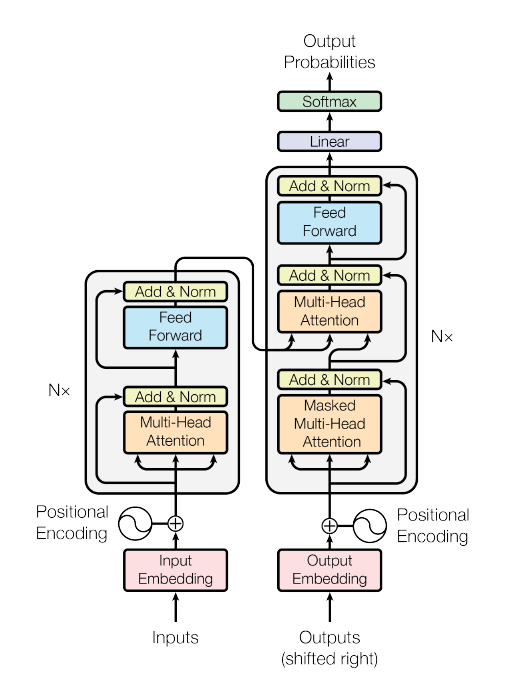
\includegraphics[width=\textwidth]{images/vanilla-arch.png}
    \caption{}
    \label{fig:vanilla-arch}
\end{subfigure}
\begin{subfigure}[b]{0.4\textwidth}
    \centering
    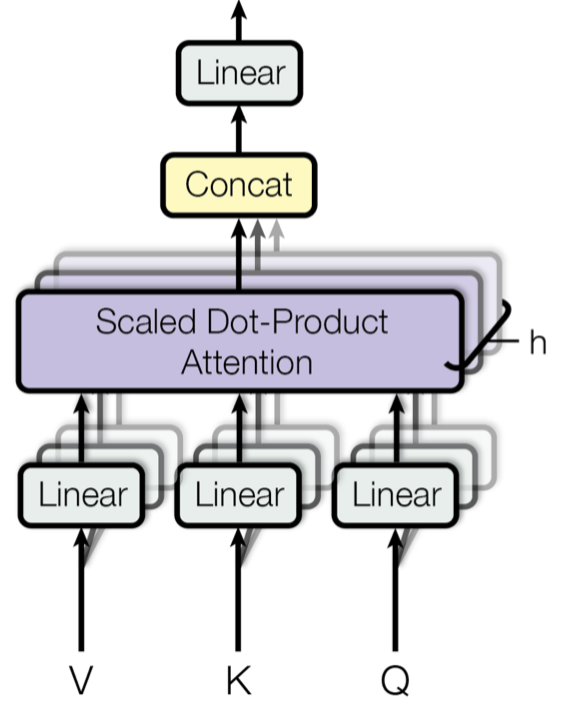
\includegraphics[width=0.9\textwidth]{images/multi-head.png}
    \caption{}
    \label{fig:multi-head}
\end{subfigure}
\caption{Transformers Architecture (a) and Multi-Head Attention (b) \cite{vaswani2023attention}}
\end{figure}

In order to describe the encoder and decoder of the Transformer architecture, we first need to understand the attention mechanisms and position-wise feed-forward layers.

\subsection{Multi-Head Attention}

Attention is the mechanism used by this architecture to capture dependencies between different positions within a sequence by attending to all positions simultaneously. Mathematically, this is represented by the function 
\begin{equation}
    A(Q, K, V) = \softmax\left(\frac{QK^\top}{\sqrt{d_k}}\right) V,
\end{equation}
where $Q \in \mathbb{R}^{m \times d_k}$ is the query matrix, $K \in \mathbb{R}^{n\times d_k}$ is the key matrix, and $V \in \mathbb{R}^{n \times d_k}$ is the value matrix. Conceptually, attention outputs the relevant values given a query to a set of key-value pairs by considering the similarity between the queries and the keys and then obtaining the values corresponding to the most similar keys. The product of $QK^T$ is scaled by $1/\sqrt{d_k}$ due to empirical observations that the unnormalized operation has values in regions of small gradients for the softmax function.

Additionally, to obtain the matrices $Q, K,$ and $V$, generally, an attention mechanism applies a linear map to the inputs $X_Q, X_K,$ and $X_V$, i.e. $Q = X_QW_Q, K=X_KW_K, V=X_VW_V$ for three learnable matrices $W_Q, W_K \in \mathbb{R}^{d \times d_k}, W_V \in \mathbb{R}^{d \times d_v} $. It is the convention to take $d_v = d_k$.


What we just described is called an \textit{Attention Head} and, as the name indicates, the multi-headed attention stacks several attention heads with unique sets of parameters in parallel. The outputs $A_1, \ldots, A_h$ of $h$ heads are then concatenated along the embedding dimension. It is the convention to set $h = d / d_k$ in order to keep the embedding dimension constant throughout the layers for easiness of stacking.

Multi-head attention has three main variants used for the encoder and decoder:
\begin{itemize}
    \item \textbf{Self-Attention:} This is the attention block used for the encoder. It sets $X_Q = X_K = X_V = X$, where $X \in \mathbb{R}^{L \times d}$ is the input of the encoder block.
    \item \textbf{Masked Self-Attention:} This is the first attention block used for the decoder. It also has $X_Q = X_K = X_V = X$ where $X \in \mathbb{R}^{M \times d}$ is the input of the decoder block, but in this variant, the positions are only allowed to attend to earlier positions in the output sequence. This is done by masking future positions to $-\infty$ before the softmax calculation.
    \item \textbf{Encoder-Decoder Attention:} This is the second attention block used for the decoder. It takes as input $X_Q$ the output of the masked self-attention (after residual connection and normalization as discussed later) and $X_K = X_V = Z$, the output of the encoder stack. This is meant to add the context of the input sequence to the decoder.
\end{itemize}


\subsection{Position-Wise Feed-Forward Network}

Attached to the output of the attention mechanisms, the Transformer architecture also includes a fully connected feed-forward network applied to each position of the input sequence separately but with the same weights. It consists of two linear layers connected by a ReLU activation. The inner-dimension is denoted by $d_{ff}$ and is generally taken as $d_{ff} = 4d$. It can still be represented by tensordot operations as:
$$
FFN(X) = ReLU(XW_1 + b_1)W_2 + b_2.
$$ 

Notice that while the attention mechanisms described above capture dependencies between positions, this block embeds positions independently.

\vspace{2em}

Now that we have introduced the two main components, we can describe the full architecture. As represented in figure \ref{fig:vanilla-arch}, both the encoder and decoder are composed of $N$ layers of identical blocks stacked. They have \textit{Add \& Norm} sub-blocks, which represent a residual connector with the input of the preceding block, followed by layer normalization \cite{ba2016layer}. After each multi-head attention of the position-wise feed-forward layer, an Add \& Norm layer is attached.
\begin{itemize}
    \item \textbf{Encoder Block:} Consists of a multi-head self-attention mechanism and a position-wise feed-forward layer.
    \item \textbf{Decoder Block:} Consists of a multi-head masked self-attention mechanism, a multi-head encoder-decoder attention mechanism as described above, and a position-wise feed-forward layer.
\end{itemize}

Although it remains to describe a few components, the key components that will be further explored during this report are highlighted until now: Attention, Encoders, and Decoders.

As for the remaining components, we first have the tokenization. It consists of the process of turning input text into raw atomic data. These raw data
correspond to the basic elements from which the model estimates meaningful interactions.
This is done by assigning an identifier to a word, a character within words or segment
of words (subwords). Starting from a large corpus of text, the tokenizer extracts the
subwords, or tokens, to use for id assignation. As a result, it retrieves a map that relates
tokens with ids. Afterwards, this map is used to tokenize sentences that serve as inputs
to the model.

Once all data is tokenized, we have embeddings for inputs and outputs (inputs for decoder) that transform the tokens to vectors of dimension $d$ with linear transformations. This embedding is added to a positional encoding to inject information about position of tokens. These are then ready to be fed to the model.

Finally, to obtain a probability distribution for the predicted next token of the sequence, the output of the last decoder layer is passed through a linear layer with softmax activation.

\subsection{Model Adaptation}

Generally, the usage of the Transformers architecture we just described can be divided into three different categories:
\begin{itemize}
    \item \textbf{Encoder-Decoder:} The full Transformer architecture. This is typically used for seq-to-seq tasks such as machine translation. 
    \item \textbf{Encoder-only:} Only the encoder part of the Transformer architecture is used, and the encoder output is generally used to embed the input sequence. This is generally used for classification tasks. Notably, the BERT \cite{devlin2019bert} family of models is an example of this.
    \item \textbf{Decoder-only:} Only an adapted decoder is used, with the removal of the Encoder-Decoder attention mechanism. This is commonly used for generative tasks. Notably, the GPT \cite{brown2020language} family of models used a decoder-only architecture.
\end{itemize}

Beyond architectural changes, a great variety of Transformer-based models introduce diverse modifications to the model pipeline. Remarkably, since the Transformer is a flexible architecture and makes few implicit prior assumptions on the input data distribution, it is generally hard to train a model on small-scale data. This issue has been widely tackled by self-supervised pre-training on large datasets \cite{devlin2019bert}\cite{brown2020language}, which allows large networks to be trained without the need to acquire expensive manually labeled data, e.g. in the case of NLP tasks. 

Two classes of pre-training tasks that have been successfully used are \textit{Fill the Blanks} and \textit{Contrastive Learning}. For the former, the task is to predict a hidden or masked part of the input sequence or reverse a permutation applied to the input, which aims to teach the model bidirectional context leveraging. The latter consists of presenting the model with three inputs, two of which are "compatible" and one other that is not; the task is then for the model to detect which two of the three are compatible. This is generally implemented by applying a transformation to the data that is desirable for the model to be invariant. An example of it is \textit{Next Sentence Prediction} which is used for BERT, which helps capture sequence-to-sequence relationships. 

In the era of Large Language Models (LLMs), pre-trained models became the standard. A single general-purpose pre-trained model on large-scale data can be leveraged by fine-tuning the model for a wide-variety of downstream tasks, which has been powering many of the industry applications of NLP.

\subsection{Computational Costs}
Now, let us analyze the computational costs of transformers. We will restrict the study to a single encoder block, for the sake of simplicity, however it easily extends to the decoder block and a stack of blocks of either. Let us use the same notation as before, with an input sequence of length $L$, embedded space of dimension $d$, $h$ attention heads, embedding space for the keys $d_k$ ($d_k h = d$), and let $M$ be the length of the output embedding. The layer normalization and residual connection have linear complexity for each head, thus both memory and computational complexity is $O(h d_k L + Ld) = O(Ld)$.

\begin{table}[ht!]
\centering
\begin{tabular}{l c c} 
 \hline
    Module & Computation & Memory \\ [0.5ex] 
 \hline
 (Masked) Self-Attention & $O(L^2d)$ & $O(Ld + hL^2)$ \\ 
 
 Encoder-Decoder Attention & $O(LMd)$ & $O(Md + hLM)$ \\
 
 FFN & $O(Ld^2)$ & $O(Ld)$ \\

 \hline
\end{tabular}
\caption{Complexity of Attentions and Position-Wise Feed-Forward}
\label{table:1}
\end{table}

Moreover, both the self-attention and position-wise feed-forward have complexities dominated by matrix multiplications. For the former, the multiplication of $\softmax(QK^\top / \sqrt{d_k})$ of shape $L \times L$  with $V$ of shape $L \times d_k$ takes $O(L^2d_k)$ operations and $O(Ld_k)$ to store the result, while computing $QK^\top$ also takes $O(L^2d_k)$ operations and requires $L^2$ of memory to store the result. Repeating this over the $h$ heads gives the complexities as described in table \ref{table:1}. Note that this simply extends to masked self-attention as the operations are essentially the same, and similarly to encoder-decoder attention.

For the position-wise feed-forward layers, assuming the convention that $d_{ff} = 4d$, the tensor-dot described before only requires $O(Ldd_{ff}) = O(Ld^2)$ operations, with $O(Ld)$ memory is sufficient to store the partial results.



\vspace{0.5em}

Now that we analyzed the costs of a single pass through a transformer layer, let us recall that during \textit{inference} we generate one token at a time. This adds a degree to the final computational order of magnitude resulting in $O(LM^2d + M^3d)$ complexity as the decoder has two types of attention. This issue can however be mitigated through clever re-utilization of computations of the previous steps, as formulated in   appendix \ref{sec:appendix}.

\vspace{0.5em}

It is important to remark that this represents the total number of computations per layer, however, these can be efficiently parallelized due to basically no sequential dependency of computations within each module. This is in stark contrast with recurrent networks, which can be argued to have better total complexity but have a higher number of sequential operations.

Moreover, although Transformers improve training speed drastically through improved parallelism, the Self-Attention module has an alarming quadratic complexity in relation to the length of the sequence in both computation and memory. 
This is prohibitive for handling large corpus of text such as codebases, articles, or books, and generally limits the scalability of the architecture. 
Although the overall architecture also has a quadratic number of computations with relation to the embedding dimension $d$, this is a constant set as a hyperparameter, while the input sequence length can be variable and for modern applications it usually holds that $L_{max} \gg d$. With this in mind, a wide variety of novel approaches have been proposed in recent years for efficient architectural modifications. Notably, we will explore two techniques for such: Linear Transformers and Quantization.
